\chapter{Префиксные суммы}\index{Prefix sums}


% TODO: возможно, нужно заменить математическую нотацию индексов на программистскую: b_i -> b[i]


\section{Определения, основы и сила полуинтервалов}\index{Prefix sums!definitions}

\begin{definition}
    \textbf{Префиксными суммами} массива $[a_0, a_1, a_2, \ldots, a_{n - 1}]$ называется массив $[b_0, b_1, b_2, \ldots, b_n]$, определяющийся следующим образом:
\begin{align*}
&    b_0 = 0\\
&    b_1 = a_0\\
&    b_2 = a_0 + a_1\\
&    b_3 = a_0 + a_1 + a_2\\
&    \ldots\\
&    b_{n - 1} = a_0 + a_1 + \ldots + a_{n - 2}\\
&    b_n = a_0 + a_1 + \ldots + a_{n - 1}
\end{align*}
\end{definition}

\begin{observation} \textbf{Сила полуинтервалов}\\
    Обратите внимание на то, что $b_i$~--- это сумма первых $i$ элементов массива $a$. Иногда префиксные суммы определяют так, что $b_i = a_0 + a_1 + \ldots + a_i$, но этот способ неудобен на практике, в чем мы убедимся далее.

    На данном примере можно познакомиться с очень важной концепцией в алгоритмах: практически всегда вместо отрезков лучше использовать полуинтервалы. К примеру, в данном случае $b_i$~--- это сумма элементов массива $a$ на полуинтервале $[0, i)$, что на практике окажется удобнее, чем хранить в $b_i$ сумму на отрезке $[0, i]$.
\end{observation}

\begin{observation}
    Также стоит помнить о том, что длина массива $b$ на один больше длины массива $a$.
\end{observation}

\begin{observation}
    Формулу для $b_i$ можно записать рекуррентно:
\begin{align*}
&    b_0 = 0\\
&    b_{i + 1} = b_{i} + a_{i}, \quad \text{где} \quad i \ge 0
\end{align*}
\end{observation}

Из рекуррентной формулы сразу становится ясно, как посчитать массив префиксных сумм за $O(n)$:

\input{queries_data_structures/prefix_sums/codes/build_prefix_sums.cpp} % TODO: test

\begin{observation}
    Обратите внимание, что элементы массива префиксных сумм~--- это суммы большого количества элементов исходного массива, поэтому будьте аккуратнее с переполнением. И вообще, на протяжении всей этой темы вы можете столкнуться с переполнением, поэтому будьте всегда начеку! Возможно, вам нужен тип \verb+long long+ вместо \verb+int+.
\end{observation}

Кроме того, есть встроенная в C++ функция \verb+std::partial_sum+, которая как раз таки считает префиксные суммы. Пример ее работы:

\input{queries_data_structures/prefix_sums/codes/build_std.cpp} % TODO: test

Обратите внимание, что сама функция \verb+partial_sum+ не оставляет нуля в начале, поэтому нам приходится делать это самим, добавляя единицу к \verb+prefixSums.begin()+.

\begin{clarification}
    У нас уже есть две интуиции для понимания $b_i$: сумма первых $i$ элементов исходного массива и сумма элементов исходного массива на полуинтервале $[0, i)$. Давайте посмотрим на еще один вариант того, как об этом можно думать. Можно представить, что элементы массива находятся в ячейках, а префиксные суммы находятся между ними~--- на перегородках. И содержат в себе суммы всего того, что находится перед этой перегородкой.

%\includegraphics[width=10cm]{queries_data_structures/prefix_sums/pictures/basic_prefix_sums_manim.png}

\

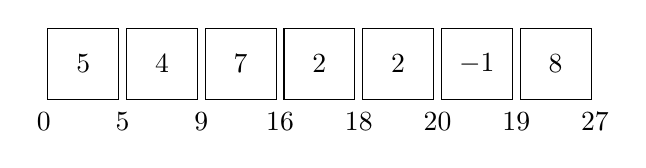
\begin{tikzpicture}
\foreach \n [count=\x] in {5, 4, 7, 2, 2, -1, 8}
  \node[rectangle, minimum size=9mm, draw] at (\x, 0) {$\n$};

\foreach \s [count=\x] in {0, 5, 9, 16, 18, 20, 19, 27}
  \node[below] at (\x-.5, -.5) {$\s$};
\end{tikzpicture}


%TODO: tikz picture

%\begin{tikzpicture}[
%    MyStyle/.style={draw, minimum width=2em, minimum height=2em, 
%                outer sep=0pt},
%  ]
%
%    %\draw[step=1cm, gray, thin] (0, 0) grid (7, 1);
%
%\matrix (A) [matrix of math nodes, nodes={MyStyle, anchor=center}, column sep=-\pgflinewidth]
%{5 & 4 & 7 & 2 & 2 & -1 & 8\\};
%
%\end{tikzpicture}

\end{clarification}

\section{Базовое применение}\index{Prefix sums!Basic applications}

Давайте сразу же применим префиксные суммы на примере задачи.

\begin{problem}
    Дан массив целых чисел, и приходят запросы вида <<найти сумму на полуинтервале с позиции $l$ до позиции $r$>>. Нужно отвечать на запросы за $\O(1)$.
\end{problem}

\begin{solution}
    Давайте изначально перед ответами на запросы предпосчитаем массив префиксных сумм. Тогда если бы во всех запросах $l$ было равно нулю, то ответом на запрос была бы просто префиксная сумма $b_{r}$.

    Но как же действовать, если $l \neq 0$? В префиксной сумме $b_{r}$ содержатся все нужные нам элементы, однако есть еще лишние: $a_0, a_1, \ldots, a_{l - 1}$. Но ведь сумма этих элементов~--- это как раз таки $b_l$. Таким образом, выполнено тождество:

$$
a_{l} + a_{l + 1} + \ldots + a_{r - 1} = b_{r} - b_{l}
$$

То есть для ответа на запрос поиска суммы на полуинтервале нужно просто вычесть друг из друга две предпосчитанные префиксные суммы.
\end{solution}

\input{queries_data_structures/prefix_sums/codes/get_query.cpp} % TODO: test

\begin{observation}
    Обратите внимание на то, какие красивые формулы у нас получаются: сумма на полуинтервале $[l, r)$~--- это $b_r - b_l$. Такая красота достигается именно благодаря тому, что мы используем полуинтервалы: и запросы у нас даны в виде полуинтервалов, и префиксные суммы. Если бы префиксные суммы были посчитаны в виде $b_i = a_0 + a_1 + \ldots + a_i$, то в формуле появились бы неприятные $\pm 1$, в которых легко запутаться: $b_r - b_{l - 1}$, и случай, когда $l = 0$, стал бы крайним, его надо было бы разбирать отдельно.
\end{observation}

\section{А что кроме суммы?}\index{Prefix sums!xor}

Давайте зададимся вопросом: для каких операций можно использовать префиксные суммы? Не только же для сложения? Какими свойствами должна обладать операция, чтобы можно было воспользоваться префиксными суммами?

На самом деле, необходимо, чтобы функция, которую мы считаем на отрезке, была обратима, что равносильно тому, что должна быть возможность по двум префиксам восстановить значение на отрезке. К примеру, операция суммы обратима, потому что если мы прибавили лишнее, потом это можно вычесть. А операции минимума и максимума необратимы. Нельзя по значениям минимумов на префиксах получить значение минимума на отрезке. К примеру, если элемент на позиции $0$ в массиве самый маленький, то все префиксные минимумы будут равны этому элементу, но минимумы на каких-то отрезках совсем с ним не связаны.

% \includegraphics[width=10cm]{queries_data_structures/prefix_sums/pictures/prefix_minimums_manim.png}

\

\begin{tikzpicture}
\foreach \n [count=\x] in {0, 4, 3, 2, 8, 2, 7}
    \ifthenelse{\x > 2 \AND \x < 7}{\node[rectangle, minimum size=9mm, blue, draw]}{\node[rectangle, minimum size=9mm, draw]} at (\x, 0) {$\n$};

\foreach \s [count=\x] in {$+\infty$, $0$, $0$, $0$, $0$, $0$, $0$, $0$}
\ifthenelse{\equal{\x}{3} \OR \equal{\x}{7}}{\node[below, rectangle, red, minimum size=4.mm, draw] at (\x-.5, -.5) {\textcolor{red}{\s}}}{\node[below] at (\x-.5, -.5) {\s}};

\draw [decorate, blue, decoration={brace}]
(2.5,0.55) -- (6.5,0.55) node [midway,above]
{\footnotesize $\min = 2$};
\end{tikzpicture}

%TODO: tikz picture

%\begin{tikzpicture}[
%    MyStyle/.style={draw, minimum width=2em, minimum height=2em, 
%                outer sep=0pt},
%  ]
%
%\matrix (A) [matrix of math nodes, nodes={MyStyle, anchor=center}, column sep=-\pgflinewidth]
%{0 & 4 & 3 & 2 & 8 & 2 & 7\\};
%
%\end{tikzpicture}

Но кроме суммы есть и другие операции, которые являются обратимыми. Одна из самых популярных~--- это, пожалуй, операция <<побитового исключающего или>>\footnote{ \href{https://learn.javascript.ru/bitwise-operators\#isklyuchayuschee-ili}{Подробнее про эту операцию можно прочитать здесь} }, которая еще называется <<\verb+xor+>> и обозначается $\oplus$.

При этом для \verb+xor+'а пользоваться префиксными суммами еще удобнее. Выполнено тождество $x \oplus x = 0$ для любого числа $x$, что означает, что операция \verb+xor+ обратна сама себе, так что формула вычисления побитового исключающего или на отрезке получается такая:

$$
a_l \oplus a_{l + 1} \oplus \ldots \oplus a_{r - 1} = b_r \oplus b_l
$$
\section{Продвинутые применения}\index{Prefix sums!Advanced applications}

Давайте решим еще пару задач, в которых нам понадобятся префиксные суммы.

\begin{problem}
    Дан массив. Необходимо за $\O(n \log n)$ найти любой его непустой подотрезок с нулевой суммой элементов.
\end{problem}

\begin{solution}
    Как мы уже знаем, суммы на отрезках~--- это разности префиксных сумм. Поэтому то, что сумма на отрезке равна нулю, равносильно тому, что префиксные суммы его концов равны.

    Таким образом, мы свели задачу нахождения подотрезка нулевой суммы к задаче нахождения двух одинаковых элементов в массиве префиксных сумм. Для этого можно, к примеру, отсортировать массив префиксных сумм и искать совпадающие элементы среди соседних.
    Либо же можно воспользоваться хеш-таблицей (\verb+unordered_map+ в C++), и тогда асимптотика решения будет вовсе $\O(n)$.
\end{solution}

\begin{exercise}
    Даны два массива одинаковой длины. Необходимо найти такой подотрезок, чтобы сумма элементов первого массива на этом подотрезке совпадала с суммой элементов второго массива на этом подотрезке. Асимптотика $\O(n)$.
\end{exercise}


\begin{problem}
    Кузнечик находится в клетке с индексом $0$ и хочет попасть в клетку с индексом $n$. За один прыжок кузнечик может переместиться на любое количество клеток вперед, но при этом не меньше $l$ и не больше $r$. Найдите, сколько существует маршрутов кузнечика. Асимптотика $\O(n)$.
\end{problem}

\begin{solution}
    Задача очень похожа на стандартную задачу о кузнечике, однако в ней прыжки имели длину $1$ и $2$, а теперь у нас количество разных прыжков не ограничено, поэтому такое же решение будет работать за $\O(n \cdot (r - l))$, что в худшем случае будет $\O(n^2)$.

    Давайте внимательно посмотрим на формулу пересчета динамики. Количество способов попасть в клетку $i$~--- это сумма количеств способов попасть во все предыдущие клетки на пути кузнечика:

$$
dp_i = dp_{i - r} + dp_{i - r + 1} + \ldots + dp_{i - l - 1} + dp_{i - l}
$$

То есть элемент массива $dp$ определяется через сумму отрезка элементов того же массива. Давайте идти по позициям в порядке возрастания и не только насчитывать массив $dp$, но и его префиксные суммы. Тогда пересчет $dp_i$ через префиксные суммы будет работать за $\O(1)$, а асимптотика всего алгоритма~--- $\O(n)$.

Таким образом, мы видим, что в задачах необязательно предпосчитывать массив префиксных сумм заранее, он может строиться по ходу решения задачи и одновременно с этим использоваться.
\end{solution}


\begin{observation} \label{prefix_sums:advanced:segment_tree}
Префиксные суммы очень удобны для подсчета суммы на отрезке в том случае, если массив в ходе запросов не меняется. Потому если какой-то элемент массива поменялся, то нужно пересчитать все префиксные суммы, в которые он входит. Это очень долго! Если есть запросы изменения, то лучше подойдут более продвинутые структуры данных: к примеру, дерево отрезков и дерево Фенвика.
\end{observation}

\section{Двумерный случай}\index{Prefix sums!2D}

Мы уже научились искать сумму на отрезке в одномерном массиве при помощи префиксных сумм, но префиксные суммы легко обобщаются и на б\'{о}льшие размерности. Давайте научимся искать сумму на прямоугольнике в двумерном массиве. Пусть нам дан двумерный массив $a_{i, j}$.
Определим его префиксные суммы так:

$$
b_{i + 1, j + 1} = \sum_{x \le i} \ \sum_{y \le j} a_{x, y} = a_{0, 0} + a_{0, 1} + a_{0, 2} + \ldots + a_{0, j} + a_{1, 0} + a_{1, 1} + \ldots + a_{1, j} + \ldots +
$$
$$
+a_{i, 0} + a_{i, 1} + \ldots + a_{i, j}
$$

Для двумерных префиксных сумм тоже полезно представлять, что они находятся между значениями исходного массива в узлах сетки и отвечают за сумму всего, что выше и левее этой точки.

Можно воспринимать происходящее, как будто мы построили префиксные суммы по одной координате, а затем посчитали префиксные суммы префиксных сумм по другой координате.

% \includegraphics[width=10cm]{queries_data_structures/prefix_sums/pictures/2d_1d_1d_manim.png}

\

\begin{tikzpicture}
\foreach \n in {0, 1, 2, 3, 4, 5}
    \foreach \col [count=\m, evaluate=\col as \prog (initially 0) using int(6 * (\m - 1) + \n + 1)] in {green, yellow, red, blue, black, black}
        \ifthenelse{\n < 3}{\node[color=\col, rectangle, minimum size=7.5mm, draw]}{\node[rectangle, minimum size=7.5mm, draw]} at (\n * 1.2, -\m * 1.2 + 1.2) {$\prog$};
    
\foreach \col [count=\x, evaluate=\col as \prog (initially 0) using int(\x * 18 - 12)] in {green, yellow, red, blue}
    \node[font=\small, color=\col] at (2.5 * 1.2, -\x * 1.2 + 1.2) {$\prog$};

\foreach \s in {1, 2, 3}
    \node[font=\small, color=purple] at (2.5 * 1.2, -\s * 1.2 + 1.2 * 0.5) {$+$};
    
\node[font=\small, color=purple] at (2.5 * 1.2, -3.25 * 1.2) {$=$};

\node[color=purple] at (2.5 * 1.2, -3.5 * 1.2) {$132$};

%    \ifthenelse{\x > 2 \AND \x < 7}{\node[rectangle, minimum size=9mm, blue, draw]}{\node[rectangle, minimum size=9mm, draw]} at (\x, 0) {$\n$};

%\foreach \s [count=\x] in {$+\infty$, $0$, $0$, $0$, $0$, $0$, $0$, $0$}
%\ifthenelse{\equal{\x}{3} \OR \equal{\x}{7}}{\node[below, rectangle, red, minimum size=4.mm, draw] at (\x-.5, -.5) {\textcolor{red}{\s}}}{\node[below] at (\x-.5, -.5) {\s}};

%\draw [decorate, blue, decoration={brace}]
%(2.5,0.55) -- (6.5,0.55) node [midway,above]
%{\footnotesize $\min = 2$};
\end{tikzpicture}

%TODO: tikz picture

Таким образом, можно насчитать префиксные суммы на одномерных массивах, а потом насчитать префиксные суммы на массивах префиксных сумм.

\input{queries_data_structures/prefix_sums/codes/2d_1d_1d_build.cpp} % TODO: TEST

Альтернативный вариант подсчета префиксных сумм~--- вновь воспользоваться рекуррентной формулой. Это будет немного сложнее, чем в одномерном случае. Формула выглядит следующим образом:

$$
b_{i + 1, j + 1} = b_{i, j + 1} + b_{i + 1, j} - b_{i, j} + a_{i, j}
$$

Эту формулу легко понять из картинки (зеленая область также принадлежит синей и желтой):

%\includegraphics[width=10cm]{queries_data_structures/prefix_sums/pictures/build_2d_manim.png}

\

%\textcolor{purple}{$?$}$=$\textcolor{blue}{$y$}$+$\textcolor{yellow}{$z$}$-$\textcolor{green}{$x$}$+$\textcolor{red}{$a[i][j]$}

$$\textcolor{purple}{?}=\textcolor{blue}{y}+\textcolor{yellow}{z}-\textcolor{green}{x}+\textcolor{red}{a[i][j]}$$

\begin{tikzpicture}
\foreach \n in {0, 1, 2, 3, 4, 5, 6, 7}
    \foreach \m in {0, 1, 2, 3, 4}
    \ifthenelse{\n < 5 \AND \m < 3}{\node[rectangle, color=green, minimum size=7.5mm, draw]}{\ifthenelse{\equal{\n}{5} \AND \m < 3}{\node[rectangle, color=blue, minimum size=7.5mm, draw]}{\ifthenelse{\equal{\m}{3} \AND \n < 5}{\node[rectangle, color=yellow, minimum size=7.5mm, draw]}{\ifthenelse{\equal{\m}{3} \AND \equal{\n}{5}}{\node[rectangle, color=red, minimum size=7.5mm, draw]}{\node[rectangle, minimum size=7.5mm, draw]}}}} at (\n * 1.2, -\m * 1.2) {};
        %\ifthenelse{\n < 3}{\node[color=\col, rectangle, minimum size=7.5mm, draw]}{\node[rectangle, minimum size=7.5mm, draw]} at (\n * 1.2, -\m * 1.2 + 1.2) {$\prog$};

\node[font=\small, color=green] at (4.5 * 1.2, -2.5 * 1.2) {$x$};
\node[font=\small, color=blue] at (5.5 * 1.2, -2.5 * 1.2) {$y$};
\node[font=\small, color=yellow] at (4.5 * 1.2, -3.5 * 1.2) {$z$};
\node[font=\small, color=purple] at (5.5 * 1.2, -3.5 * 1.2) {$?$};
 \end{tikzpicture}

\

% TODO: tikz picture

Мы берем сумму двух меньших префиксных сумм, которые накрывают нашу, однако их пересечение учтется дважды, поэтому его надо вычесть. Но ведь это пересечение~--- это и есть $b_{i, j}$. И в конце стоит не забыть прибавить новый элемент~--- $a_{i, j}$.

Элементы, через которые мы считаем $b_{i + 1, j + 1}$ имеют меньшие индексы, поэтому подсчет двумерных префиксных сумм можно вести просто двумя вложенными циклами по возрастанию.

\input{queries_data_structures/prefix_sums/codes/2d_build.cpp} % TODO: TEST

Теперь пускай нам надо найти сумму на <<полупрямоугольнике>> (двумерный полуинтервал) с противоположными углами в точках $(lx, ly)$ и $(rx, ry)$ (левые границы~--- включительно, правые~--- исключительно). Сумма элементов на этом полупрямоугольнике будет выражаться так:
$$
\sum_{lx \le i < rx} \ \sum_{ly \le j < ry} a_{i, j} = b_{rx, ry} - b_{lx, ry} - b_{rx, ly} + b_{lx, ly}
$$

Эту формулу также легче понимать, смотря на картинку:

%\includegraphics[width=10cm]{queries_data_structures/prefix_sums/pictures/find_2d_manim.png}

\

$$sum=\textcolor{purple}{b[rx][ry]}-\textcolor{blue}{b[lx][ry]}-\textcolor{yellow}{b[rx][ly]}+\textcolor{green}{b[lx][ly]}$$

\begin{tikzpicture}
\foreach \n in {0, 1, 2, 3, 4, 5, 6, 7, 8, 9, 10, 11, 12, 13, 14}
    \foreach \m in {0, 1, 2, 3, 4, 5, 6, 7}
    \ifthenelse{\n > 5 \AND \n < 12 \AND \m > 1 \AND \m < 6}{\node[rectangle, color=purple, minimum size=4.5mm, draw]}{\node[rectangle, minimum size=4.5mm, draw]} at (\n * 0.7, -\m * 0.7) {};

\draw[color=orange, thick] (5.5 * 0.7, -1.5 * 0.7) -- (5.5 * 0.7, -5.5 * 0.7) -- (11.5 * 0.7, -5.5 * 0.7) -- (11.5 * 0.7, -1.5 * 0.7) -- cycle;

\node[circle, fill=green, draw, inner sep=1.7pt, color=green] at (5.5 * 0.7, -1.5 * 0.7) {};
\node[circle, fill=yellow, draw, inner sep=1.7pt, color=yellow] at (5.5 * 0.7, -5.5 * 0.7) {};
\node[circle, fill=blue, draw, inner sep=1.7pt, color=blue] at (11.5 * 0.7, -1.5 * 0.7) {};
\node[circle, fill=purple, draw, inner sep=1.7pt, color=purple] at (11.5 * 0.7, -5.5 * 0.7) {};

\draw[->] (-0.4, -0.3) -- (-0.4, -0.3 - 6 * 0.7) node [midway, left] (TextNode) {$x$};
\draw[->] (-0.4 + 0.7, -0.5 - 7 * 0.7) -- (-0.4 + 0.7 * 14, -0.5 - 7 * 0.7) node [midway, below] (TextNode2) {$y$};
 \end{tikzpicture}



%TODO: tikz picture

Сначала мы взяли большой прямоугольник, который накрывает нужный нам, потом удалили ненужное слева и сверху, но то, что находится на их пересечении, мы удалили дважды, так что надо вернуть это пересечение назад.

\begin{observation}
    Именно в двумерном случае, а также больших размерностях становится видна мощь полуинтервалов. В формуле нет ни одной цифры ($\pm 1$). Мы просто берем префиксные суммы на краях и складываем и вычитаем их.

    Если бы мы определяли $b_{i, j}$ как сумму на отрезке, то есть $\sum_{x \le i} \sum_{y \le j} a_{x, y}$, то формула для суммы на прямоугольнике выглядела бы следующим образом:

$$
b_{rx, ry} - b_{lx - 1, ry} - b_{rx, ly - 1} + b_{lx - 1, ly - 1}
$$

Вероятность написать эти формулы правильно постепенно стремится к нулю.
\end{observation}



\section{Трехмерный случай}\index{Prefix sums!3D}

Мы разобрались с двумерным случаем, теперь пойдем еще дальше! Префиксные суммы на трехмерном массиве определяются аналогично:

$$
b_{i + 1, j + 1, k + 1} = \sum_{x \le i} \ \sum_{y \le j} \ \sum_{z \le k} a_{x, y, z}
$$

Рекурентная формула для их подсчета будет такая:

$$
b_{i + 1, j + 1, k + 1} = b_{i, j + 1, k + 1} + b_{i + 1, j, k + 1} + b_{i + 1, j + 1, k} - b_{i + 1, j, k} - b_{i, j + 1, k} - b_{i, j, k + 1} + b_{i, j, k} + a_{i, j, k}
$$

И для поиска суммы на <<полупараллелепипеде>> (трехмерном полуинтервале) с противоположными углами в точках $(lx, ly, lz)$ и $(rx, ry, rz)$ подойдет следующая формула:

$$
\sum_{lx \le i < rx} \ \sum_{ly \le j < ry} \ \sum_{lz \le k < rz} a_{i, j, k} = b_{rx, ry, rz} - b_{lx, ry, rz} - b_{rx, ly, rz} - b_{rx, ry, lz} + b_{rx, ly, lz} + b_{lx, ry, lz} + b_{lx, ly, rz} - b_{lx, ly, lz}
$$

Формулы страшные! Но показываю я вам их для того, чтобы сформулировать правила, по которым они работают в общем случае для любой размерности. Потому что если у вас есть пространственное мышление, то по картинке придумать формулу для трехмерного случая вы еще сможете, а вот для четырехмерного уже вряд ли.

\begin{theorem}
    В рекуррентной формуле подсчета префиксных сумм мы берем комбинацию всех возможных вариантов вычитания единиц из индексов. При этом если мы вычли нечетное количество единиц, то слагаемое идет с плюсом, а если четное, то с минусом. В конце нужно не забыть еще прибавить один новый элемент изначального массива $a$.

    Понять, почему именно нечетное с плюсом, можно по тому, что мы точно знаем, что слагаемые, в которых всего из одной координаты вычли единицу, должны идти с плюсом, ведь при их помощи мы накрываем изначально нашу префиксную сумму, а потом уже остальными пытаемся ее корректировать.
\end{theorem}

\begin{theorem}
    Аналогичное правило есть и для формулы поиска суммы на полупараллелепипеде. Берется сумма всевозможных комбинаций левых и правых границ по каждой координате, при этом если левых границ четное количество, то слагаемое берется с плюсом, а если нечетное, то с минусом.

    Опять же, понять, почему именно четное с плюсом, а нечетное с минусом, очень легко: слагаемое, в котором все границы правые~--- это самое большое слагаемое, которое мы потом корректируем, так что оно точно должно быть с плюсом.
\end{theorem}

\begin{exercise}
    При помощи этих двух незатейливых правил попробуйте составить формулы для построения префиксных сумм и поиска суммы на\\(полу)гиперпрямоугольнике в четырехмерном пространстве.
\end{exercise}

\begin{observation}
    Трехмерный префиксный массив можно насчитать другим способом так же как и двумерный: сначала посчитать одномерные префиксные суммы, потом на них насчитать двумерные и затем уже на них посчитать трехмерные.
\end{observation}

\begin{observation}
    Если вы знаете, что такое формула включений-исключений, то в каком-то смысле именно она и применяется при построении и при ответе на запросы в многомерных префиксных суммах.
\end{observation}


\section{Разностный массив}\index{Prefix sums!Difference}

Мы уже научились по массиву строить его массив префиксных сумм. А теперь давайте научимся по массиву префиксных сумм строить исходный массив, то есть применять обратную операцию.

\begin{definition}
    \textbf{Разностным массивом} массива $[b_0, b_1, \ldots, b_{n - 1}]$ называется массив $[a_0, a_1, \ldots, a_{n - 2}]$, определяющийся следующим образом:

\begin{align*}
&   a_0 = b_1 - b_0\\
&   a_1 = b_2 - b_1\\
&   a_2 = b_3 - b_2\\
&   \ldots\\
&   a_{n - 3} = b_{n - 2} - b_{n - 3}\\
&   a_{n - 2} = b_{n - 1} - b_{n - 2}
\end{align*}
\end{definition}

Очевидно, что если $b$~--- массив префиксных сумм массива $a$, то массив $a$~--- разностный массив массива $b$, потому что формула $a_i = b_{i + 1} - b_i$~--- это просто преобразованная рекуррентная формула для поиска префиксных сумм: $b_{i + 1} = b_i + a_i$.
Однако разностный массив может помочь нам даже там, где массивом префиксных сумм и не пахнет!
Также обратите внимание, что если для подсчета массива префиксных сумм была нужна рекуррентная формула, то каждый член разностного массива зависит всего от двух элементов исходного, так что можно пользоваться формулами из определения для подсчета разностного массива за $\O(n)$.

\input{queries_data_structures/prefix_sums/codes/build_diffs_array.cpp} % TODO: TEST

\begin{observation}
    Если вы знакомы с основами матанализа, можно заметить, что переход к разностному массиву~--- это дискретное дифференцирование, а переход к массиву префиксных сумм~--- дискретное интегрирование.
\end{observation}


\section{Применения разностного массива}\index{Prefix sums!Difference apply}

Решим несколько задач, используя разностный массив. Мы уже решили задачу нахождения суммы на отрезке при помощи префиксных сумм, а теперь рассмотрим в некотором смысле обратную задачу: задачу о прибавлении на отрезке.

\begin{problem}
    Дан массив длины $n$. Приходят $q$ запросов: прибавить на полуинтервале $[l, r)$ ко всем элементам число $d$. После выполнения всех запросов необходимо вывести получившийся массив. Асимптотика $\O(n + q)$.
\end{problem}

\begin{solution}
    В замечании \ref{prefix_sums:advanced:segment_tree} мы говорили о том, что если элементы массива меняются, то для решения задачи понадобятся продвинутые структуры, такие как дерево отрезков или дерево Фенвика. Однако здесь мы обойдемся без них, потому что у нас есть только запросы изменения, а запрос <<получения>> есть только один в самом конце.

    Давайте в начало исходного массива $b$ допишем фиктивный элемент ноль и у получившегося массива возьмем разностный массив $a$. После чего будем наблюдать за тем, как этот массив $a$ будет меняться в следствии запросов изменения массива $b$ на отрезке.
    Фиктивный ноль мы добавили для того, чтобы не потерять информацию о нулевом элементе массива $b$, ведь только по разностям соседних элементов восстановить исходный массив не получится.

    Пускай на полуинтервале $[l, r)$ исходного массива (или на полуинтервале $[l + 1, r + 1)$ массива с фиктивным нулем в начале) прибавили ко всем элементам $d$.
    Заметим, что элементы массива $a$ на позициях меньших $l$ и больших $r$ никак не поменяются, потому что оба элемента в разности никак не поменялись. На позициях $l + 1, \ldots, r - 1$ тоже ничего не поменяется, потому что к обоим элементам разности прибавят $d$, в результате чего сама разность не изменится. К примеру, для позиции $l + 1$:

$$
b^{new}_{l + 1} - b^{new}_{l} = \left(b^{old}_{l + 1} + d\right) - \left(b^{old}_l + d\right) = b^{old}_{l + 1} + d - b^{old}_l - d = b^{old}_{l + 1} - b^{old}_l
$$

Таким образом, после операции прибавления на отрезке изменятся только два элемента разностного массива: $a_{l}$ заменится на $a_{l} + d$, и $a_r$ заменится на $a_r - d$.

Алгоритм получается следующий: изначально перейдем от исходного массива к его разностному массиву, предварительно добавив в начало массива $0$, чтобы не потерять информацию о $b_0$.
Затем выполняем операции изменения за $\O(1)$ каждую, потому что нужно поменять каждый раз всего два элемента. И в конце нужно вернуться к исходному виду массива, посчитав префиксные суммы.
\end{solution}

\input{queries_data_structures/prefix_sums/codes/add_on_segment.cpp} % TODO: TEST

\begin{observation}
    Обратите внимание на то, что если $r = n$, то такого элемента нет в массиве $a$, ведь этот элемент отвечал бы за разность элемента после конца массива $b$ с последним элементом массива $b$, которая нас не интересует. Поэтому в таком случае мы ничего не делаем.
\end{observation}

\begin{observation}
    На самом деле можно было даже не брать разностный массив. Можно было считать, что изначально массив состоял из всех нулей, тогда его разностный массив тоже состоит из всех нулей; на этом массиве произвести все операции, посчитать массив префиксных сумм и уже в самом конце прибавить начальные значения элементов массива.
\end{observation}

\begin{problem}
    Дан массив длины $n$. Приходят $q$ запросов: прибавить на полуинтервале $[l, r)$ арифметическую прогрессию с шагом $step$, то есть к элементу на позиции $l$ прибавить $step$, к элементу на позиции $l + 1$ прибавить $2 \cdot step$, к элементу на позиции $l + 2$ прибавить $3 \cdot step$, \ldots, и наконец к элементу на позиции $r - 1$ прибавить $\left(r - l\right) \cdot step$.

    После выполнения всех запросов необходимо вывести получившийся массив. Асимптотика $\O(n + q)$.
\end{problem}

\begin{solution}
    Задача похожа на предыдущую, но явно сложнее, ведь к каждому элементу на отрезке прибавляется разное число.
    Давайте посмотрим, что произойдет, если мы как и раньше перейдем к разностному массиву.
    Заметим, что если мы на полуинтервале прибавили $step, 2 \cdot step, \ldots, (r - l) \cdot step$, то в разностном массиве мы на некотором полуинтервале прибавим ко всем элементам $step$, а также из элемента на правой границе вычтется $(r - l) \cdot step$. Но ведь прибавлять число на отрезке мы уже умеем! Давайте перейдем к разностному массиву разностного массива, при этом не забыв в таком случае добавить уже не один, а два фиктивных нуля в начало массива. Тогда для разностного массива разностного массива изменятся только элементы на позициях $l$, $r$ и $r + 1$, так что мы можем выполнять все операции за $\O(1)$, а затем в конце дважды насчитать массив префиксных сумм, вернувшись к исходному массиву.
\end{solution}

\input{queries_data_structures/prefix_sums/codes/add_arithm_on_segment.cpp} % TODO: test

\begin{exercise}
    Попробуйте решить последнюю задачу, если первый член арифметической прогрессии не совпадает с шагом, то есть на полуинтервале прибавляются числа $start, start + step, start + 2 \cdot step, \ldots, start + \left(r - l - 1\right) \cdot step$.
\end{exercise}

\begin{exercise}
    Как обобщить решение прошлой задачи на случай, когда на отрезке прибавляется не линейная, а квадратичная функция?
    То есть прибавляются числа $step, 4 \cdot step, 9 \cdot step, \ldots, (r - l)^2 \cdot step$.
\end{exercise}

\begin{exercise}
    Представьте, что у вас есть список операций виде <<прибавить на полуинтервале $[l, r)$ значение $d$>>. Но вам нужно выполнять не эти операции, а целые отрезки операций! То есть в действительности операция имеет вид <<примените к массиву операции с номерами от $L$-й до $R$-й>>.
    В конце нужно вывести получившийся массив.
    Как решать такую задачу за $\O(n + q)$?
\end{exercise}

\begin{observation}
    Если вы знаете основы матанализа, можно легко понять, почему мы производили именно такие манипуляции. Ведь если взять производную, то прибавление константы на отрезке превратится в прибавление тождественного нуля, а для линейной функции нужно взять вторую производную.
\end{observation}


\section{Двумерный разностный массив}\index{Prefix sums!2D difference array}

\begin{problem}
    Дан двумерный массив размера $n \times m$, изначально состоящий из всех нулей. Приходит $q$ запросов прибавления константы на прямоугольнике. В конце нужно вывести элементы получившегося массива.
\end{problem}

\begin{solution}
    Это двумерная версия задачи, которую мы рассматривали ранее, но для простоты изначальный массив состоит из нулей, поэтому нам не нужно переходить к разностному массиву. Надо подумать, к каким элементам что надо прибавить на разностном массиве, чтобы на исходном массиве прибавить $d$ на полупрямоугольнике $[lx, rx) \times [ly, ry)$.

Можно заметить, что если в разностном массиве к какому-то элементу прибавить $d$, то в исходном массиве $d$ прибавится ко всем элементам на \textbf{суффиксном} подпрямоугольнике.

%\includegraphics[width=10cm]{queries_data_structures/prefix_sums/pictures/suffix_2d_manim.png}

\

\begin{tikzpicture}
\foreach \n in {0, 1, 2, 3, 4, 5, 6, 7, 8, 9}
    \foreach \m in {0, 1, 2, 3, 4, 5}
    \ifthenelse{\n > 4 \AND \m > 2}{\node[rectangle, color=red, minimum size=6mm, draw]}{\node[rectangle, minimum size=6mm, draw]} at (\n, -\m) {};


\node[color=red] at (4.5, -2.5) {$+d$};
\end{tikzpicture}

%TODO: tikz picture

Теперь перед нами стоит задача <<прибавить на подпрямоугольнике через прибавления на суффиксных подпрямоугольниках>>. Эта задача аналогична задаче поиска суммы на подпрямоугольнике.


%\includegraphics[width=10cm]{queries_data_structures/prefix_sums/pictures/add_on_rectangle_manim.png}

\

\begin{tikzpicture}
\foreach \n in {0, 1, 2, 3, 4, 5, 6, 7, 8, 9}
    \foreach \m in {0, 1, 2, 3, 4, 5}
    \ifthenelse{\n > 3 \AND \m > 0}{\ifthenelse{\n > 6}{\ifthenelse{\m > 4}{\node[rectangle, color=blue, minimum size=6mm, draw]}{\node[rectangle, color=purple, minimum size=6mm, draw]}}{\ifthenelse{\m > 4}{\node[rectangle, color=yellow, minimum size=6mm, draw]}{\node[rectangle, color=red, minimum size=6mm, draw]}}}{\node[rectangle, minimum size=6mm, draw]} at (\n, -\m) {};

\draw[color=green] (3.5, -0.5)-- (3.5, -4.5) -- (6.5, -4.5) -- (6.5, -0.5)-- cycle;

\node[color=red] at (3.5, -0.5) {$+d$};
\node[color=yellow] at (3.5, -4.5) {$-d$};
\node[color=purple] at (6.5, -0.5) {$-d$};
\node[color=blue] at (6.5, -4.5) {$+d$};

\end{tikzpicture}

% TODO: tikz picture

Прибавляем мы к тем же самым клеткам, сумму которых мы брали в задаче поиска суммы на подпрямоугольнике.


В конце мы возьмем префиксные суммы получившегося двумерного массива, и это и будет ответом.

\end{solution}

\input{queries_data_structures/prefix_sums/codes/add_on_rectangle.cpp} % TODO: test

\begin{observation}
    Как и раньше, мы добавляем нули в начало. В случае двумерного массива мы добавили строку и столбец нулей. В качестве упражнения остается проверить, что индексы, к которым надо прибавлять, будут именно такие. При этом как и в одномерном случае, правые индексы могут не существовать в массиве \verb+diffs+, если они равны высоте или ширине изначального массива.
\end{observation}

\begin{exercise}
    Спросите себя: понимаете ли вы, что делать, если изначально массив состоит не из нулей?
\end{exercise}

\begin{exercise}
    Как обобщить решение предыдущей задачи, если массив уже не двумерный, а трехмерный, и прибавлять надо на параллелепипеде?
\end{exercise}

\begin{definition}
    Строго говоря, разностный двумерный массив можно строить так же, как и одномерный. Формула для его элементов будет такая:

    $$a_{i + 1, j + 1} = b_{i + 1, j + 1} - b_{i, j + 1} - b_{i + 1, j} + b_{i, j}$$

    что похоже на аналогичную формулу для двумерных префиксных сумм. Но как вы видели, на практике нам не надо изначально строить разностный массив. Нужно просто изначально считать, что он заполнен нулями, а после выполнения операций по нему посчитать массив префиксных сумм. И начальные элементы добавить уже в самом конце.
\end{definition}


\section{Задачи для практики}

\begin{itemize}
    \item Предлагается прорешать специально подготовленный \href{https://codeforces.com/group/1rv4rhCsHp/contest/319055}{контест} на codeforces. Если у вас нет доступа к соревнованию, нужно сначала вступить в \href{https://codeforces.com/group/1rv4rhCsHp/contests}{группу}.
\end{itemize}
